\documentclass[11pt,a4paper]{article}

\usepackage[utf8]{inputenc}
\usepackage[margin=0.85in]{geometry}
\usepackage{amsmath,amssymb}
\usepackage{booktabs}
\usepackage{tabularx}
\usepackage{graphicx}
\usepackage{hyperref}
\usepackage{enumitem}
\usepackage{listings}
\usepackage{xcolor}

\hypersetup{
    colorlinks=true,
    linkcolor=blue!75!black,
    urlcolor=blue!75!black,
    citecolor=blue!75!black
}

\setlist[itemize]{noitemsep, topsep=2pt}
\setlist[enumerate]{noitemsep, topsep=2pt}

\lstset{
    basicstyle=\ttfamily\footnotesize,
    breaklines=true,
    frame=single,
    backgroundcolor=\color{gray!8},
    rulecolor=\color{gray!30},
    keywordstyle=\color{blue!80!black}\bfseries,
    commentstyle=\color{green!50!black}\itshape,
    stringstyle=\color{red!60!black},
    numbers=none
}

\title{\textbf{ESP32 Digital Signature Micro-Benchmark}\\[0.2em]\large Phase A: Isolated Cryptographic Evaluation (No Network Overhead)\\[0.2em]\normalsize FYP Documentation: Embedded VPN Client (Deliverable 2)}
\author{Department of Computer Engineering}
\date{October 2026}

\begin{document}

\maketitle

\section{Phase A: Isolated Micro-Benchmarks (No Network Overhead)}

Phase~A evaluates the isolated, raw cryptographic execution of three digital signature algorithms directly on an ESP32 microcontroller at an equivalent 128-bit classical security baseline. All tests execute entirely within local static and dynamic RAM without Wi-Fi or TCP transport latency to establish baseline hardware performance, memory consumption, and frame overhead:
\begin{enumerate}
    \item \textbf{Ed25519:} Modern Twisted Edwards Curve25519 digital signature algorithm implemented via the optimized Libsodium cryptographic library.
    \item \textbf{ECDSA P-256:} Standard NIST prime curve \texttt{secp256r1} digital signature scheme implemented via ESP32 Mbed~TLS.
    \item \textbf{Classical RSA-3072:} Classical Rivest-Shamir-Adleman algorithm configured with a 3072-bit modulus, PKCS\#1 v1.5 padding, and SHA-256 implemented via ESP32 Mbed~TLS.
\end{enumerate}

\subsection{Microcontroller Test Environment}

\begin{itemize}
    \item \textbf{Microcontroller Hardware:} Espressif ESP32-D0WDQ6 (Revision v1.0), Dual-Core Xtensa LX6.
    \item \textbf{Processor Clock Frequency:} 240~MHz ($240,000,000\text{ cycles/second}$).
    \item \textbf{Available Static/Dynamic SRAM:} $\sim 329\text{ KB}$ free heap at benchmark startup.
    \item \textbf{Cycle-Accurate Measurement:} Read directly from the Xtensa hardware 32-bit cycle register (\texttt{ccount}). Because the clock operates at a fixed 240~MHz:
    \begin{equation}
    \text{Latency (ms)} = \frac{\text{Hardware CPU Cycles}}{240,000}
    \end{equation}
\end{itemize}

\section{Key Performance Indicators (KPIs)}

The evaluation profiles seven Key Performance Indicators (KPIs) covering execution latency, hardware workload, wire payload footprint, and dynamic RAM consumption:

\subsection{KPI Definitions and Operational Impact}

\begin{itemize}
    \item \textbf{SIG-1 (Key Generation Latency):} Hardware cycles and elapsed milliseconds required to generate a fresh asymmetric keypair (public and private key). Crucial if ephemeral client authentication keys are generated per VPN session.
    \item \textbf{SIG-2 (Public Key Wire Size):} Size in bytes of the serialized public key exchanged during mutual identity establishment.
    \item \textbf{SIG-3 (Message Signing Latency):} Hardware cycles and elapsed milliseconds to sign a 64-byte cryptographic authentication challenge. Directly determines client response latency.
    \item \textbf{SIG-4 (Signature Wire Size):} Byte length of the generated signature transmitted over the network in authentication response frames.
    \item \textbf{SIG-5 (Verification Latency):} Hardware cycles and elapsed milliseconds to verify the peer's digital signature on a 64-byte challenge. Governs gateway authentication processing time.
    \item \textbf{SIG-6 (Total Client Sign Time):} Total on-chip processor execution latency ($\text{SIG-1} + \text{SIG-3}$) required for complete client-side key setup and challenge signing.
    \item \textbf{SIG-7 (Peak Dynamic Heap Memory):} Maximum dynamic RAM allocated from the ESP32 heap during cryptographic execution. Minimizing dynamic allocation is critical to prevent heap fragmentation and Out-Of-Memory (OOM) crashes in memory-constrained IoT nodes.
\end{itemize}

\subsection{Iteration Count and Statistical Reliability Strategy}

\begin{itemize}
    \item \textbf{Fast Benchmark Iterations ($N = 100$):} For Ed25519, ECDSA P-256, and fast RSA signing/verification, 100 independent iterations were measured to compute stable arithmetic means and eliminate OS scheduling artifacts.
    \item \textbf{RSA Key Generation Iterations ($N = 10$):} Because 3072-bit RSA key generation requires stochastic prime searching across thousands of Miller-Rabin tests (taking $\sim 9.6\text{ seconds}$ per key), 10 iterations were executed with watchdog yield intervals (\texttt{vTaskDelay(1)}) to avoid triggering the ESP32 Task Watchdog Timer (TWDT).
\end{itemize}

\begin{table}[htbp]
\centering
\small
\caption{Summary of Digital Signature Benchmarking KPIs}
\label{tab:sig_kpis}
\begin{tabularx}{\textwidth}{lll X}
\toprule
\textbf{KPI ID} & \textbf{Metric Name} & \textbf{Unit} & \textbf{Operational Significance for Embedded VPN} \\
\midrule
\textbf{SIG-1} & Key Generation Time    & ms / cycles & Ephemeral identity generation speed \\
\textbf{SIG-2} & Public Key Wire Size   & Bytes       & Bandwidth overhead of client identity advertisement \\
\textbf{SIG-3} & Message Signing Time   & ms / cycles & Time required to sign challenge nonce during handshake \\
\textbf{SIG-4} & Signature Wire Size    & Bytes       & Bandwidth overhead of authentication challenge proof \\
\textbf{SIG-5} & Verification Time      & ms / cycles & Peer verification latency \\
\textbf{SIG-6} & Total Client Sign Time & ms / cycles & Complete client-side crypto latency ($\text{SIG-1} + \text{SIG-3}$) \\
\textbf{SIG-7} & Peak Dynamic Heap RAM  & Bytes       & Peak RAM allocated from heap during operation \\
\bottomrule
\end{tabularx}
\end{table}

\section{Benchmark Results and Comparison}

\subsection{Empirical Performance Comparison}

Table~\ref{tab:comparison_summary} presents the empirical measurements captured directly from the ESP32 serial console across all three signature schemes at 240~MHz.

\begin{table}[htbp]
\centering
\footnotesize
\setlength{\tabcolsep}{2.0pt}
\caption{Performance Comparison: Ed25519 vs. ECDSA P-256 vs. Classical RSA-3072}
\label{tab:comparison_summary}
\begin{tabular}{l c c c c c}
\toprule
\textbf{Metric} & \textbf{Ed25519} & \textbf{ECDSA P-256} & \textbf{RSA-3072} & \textbf{Winner} & \textbf{Performance Factor} \\
\midrule
\multicolumn{6}{l}{\textbf{Execution Latency (Milliseconds)}} \\
Key Generation Time (SIG-1)     & \textbf{8.56 ms}   & 146.93 ms  & 9,630.80 ms  & \textbf{Ed25519} & $17.2\times$ faster than P-256 \\
Message Signing Time (SIG-3)    & \textbf{9.42 ms}   & 158.58 ms  & 375.81 ms    & \textbf{Ed25519} & $16.8\times$ faster than P-256 \\
Verification Time (SIG-5)       & 19.80 ms           & 313.88 ms  & \textbf{1.71 ms} & \textbf{RSA-3072} & $15.9\times$ faster than P-256 \\
Total Client Sign Time (SIG-6)  & \textbf{17.99 ms}  & 305.51 ms  & 10,006.61 ms & \textbf{Ed25519} & $17.0\times$ faster than P-256 \\
\midrule
\multicolumn{6}{l}{\textbf{Hardware CPU Workload (Cycles @ 240 MHz)}} \\
KeyGen Cycles                   & \textbf{2,055,308} & 35,262,354 & 2,311,393,015 & \textbf{Ed25519} & Lowest compute cycles \\
Signing Cycles                  & \textbf{2,261,378} & 38,059,479 & 90,194,354    & \textbf{Ed25519} & Lowest compute cycles \\
Verification Cycles             & 4,750,949          & 75,331,369 & \textbf{410,321} & \textbf{RSA-3072} & Shortest verification \\
Total Client Cycles             & \textbf{4,316,686} & 73,321,833 & 2,401,587,369 & \textbf{Ed25519} & Lowest total workload \\
\midrule
\multicolumn{6}{l}{\textbf{Communication Wire Footprint (Bytes)}} \\
Public Key Wire Size (SIG-2)    & \textbf{32 bytes}  & 65 bytes   & 384 bytes     & \textbf{Ed25519} & $12.0\times$ smaller than RSA \\
Signature Wire Size (SIG-4)     & \textbf{64 bytes}  & 71 bytes   & 384 bytes     & \textbf{Ed25519} & $6.0\times$ smaller than RSA \\
Total Wire Size (Key + Sig)     & \textbf{96 bytes}  & 136 bytes  & 768 bytes     & \textbf{Ed25519} & $8.0\times$ smaller than RSA \\
\midrule
\multicolumn{6}{l}{\textbf{Memory Utilization}} \\
Peak Dynamic Heap (SIG-7)       & \textbf{108 bytes} & 300 bytes  & 2,068 bytes   & \textbf{Ed25519} & $19.1\times$ less heap than RSA \\
\bottomrule
\end{tabular}
\end{table}

\section{Selection Rationale for Ed25519}

Ed25519 is unequivocally selected as the primary mutual authentication and digital signature algorithm for the embedded VPN client based on four critical engineering justifications:

\begin{enumerate}
    \item \textbf{Superior Client Execution Speed ($17\times$ faster than ECDSA P-256):}  
    Ed25519 completes key generation in \textbf{8.56~ms} and challenge signing in \textbf{9.42~ms}, resulting in a total client cryptographic workload of only \textbf{17.99~ms}. In contrast, ECDSA P-256 requires \textbf{305.51~ms} ($17.0\times$ slower) and RSA-3072 requires \textbf{10,006.61~ms} ($\approx 10\text{ seconds}$, $556\times$ slower). Completing client-side authentication in under 20~ms minimizes device active state and preserves battery longevity.

    \item \textbf{Minimal Transmission Wire Overhead ($8\times$ smaller than RSA-3072):}  
    Ed25519 features extremely compact cryptographic representations: 32 bytes for the public key and 64 bytes for the signature, yielding an aggregate wire overhead of just \textbf{96 bytes}. ECDSA requires 136 bytes (using 65-byte uncompressed points and 71-byte ASN.1 DER signatures), while RSA-3072 requires \textbf{768 bytes}. The compact 96-byte payload avoids TCP packet segmentation and reduces Wi-Fi radio transmission time.

    \item \textbf{Ultra-Low Dynamic RAM Consumption (108 bytes vs. 2,068 bytes):}  
    The ESP32 allocates only \textbf{108 bytes} of dynamic heap memory during Ed25519 signature operations via Libsodium. ECDSA P-256 allocates 300 bytes for its point multiplication context, while RSA-3072 allocates \textbf{2,068 bytes} to maintain multi-precision integer (MPI) BigNum arithmetic structures. Ed25519 prevents heap fragmentation across prolonged uptime.

    \item \textbf{Constant-Time Execution and Immunity to Side-Channel Attacks:}  
    Ed25519 operations over Twisted Edwards Curve25519 are inherently constant-time, eliminating timing and cache side-channel vulnerabilities. In contrast, standard ECDSA implementations require high-entropy per-signature secret nonces ($k$); any bias or leakage in $k$ exposes the private key. Ed25519 derives its nonce deterministically ($r = H(\text{hash\_prefix} \parallel M)$), completely eliminating catastrophic nonce collisions.

    \item \textbf{Impracticality of Classical RSA-3072 on Embedded Clients:}  
    While RSA-3072 achieves rapid verification (\textbf{1.71~ms}) due to its small public exponent ($e = 65537$), this benefit is entirely asymmetric and serves only the verifying gateway. On the embedded client side, RSA-3072 suffers from an unviable $\sim 9.6\text{-second}$ key generation time, $375.81\text{ ms}$ signing latency, 768-byte wire overhead, and 2~KB heap allocation, rendering it inappropriate for resource-constrained IoT endpoints.
\end{enumerate}

\section{Serial Monitor Output Verification}

The serial captures below verify the empirical test executions recorded directly on the ESP32 hardware:

\subsection{Ed25519 Benchmark Execution Capture}

Figure~\ref{fig:term_ed25519} displays the serial monitor output for Ed25519 over 100 runs, demonstrating 8.56~ms keygen, 9.42~ms signing, 19.80~ms verification, and 108~bytes peak heap RAM.

\begin{figure}[htbp]
\centering
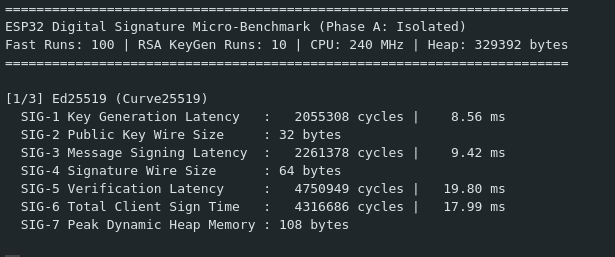
\includegraphics[width=0.85\textwidth]{screenshots/terminal_ed25519.png}
\caption{ESP32 Serial Output for Ed25519 micro-benchmarks (100 runs @ 240 MHz).}
\label{fig:term_ed25519}
\end{figure}

\subsection{ECDSA P-256 Benchmark Execution Capture}

Figure~\ref{fig:term_ecdsa} displays the serial monitor output for ECDSA P-256 over 100 runs, recording 146.93~ms keygen, 158.58~ms signing, 313.88~ms verification, and 300~bytes peak heap RAM.

\begin{figure}[htbp]
\centering
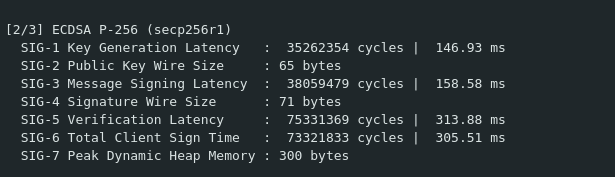
\includegraphics[width=0.85\textwidth]{screenshots/terminal_ecdsa.png}
\caption{ESP32 Serial Output for ECDSA P-256 micro-benchmarks (100 runs @ 240 MHz).}
\label{fig:term_ecdsa}
\end{figure}

\subsection{Classical RSA-3072 Benchmark Execution Capture}

Figure~\ref{fig:term_rsa} displays the serial monitor output for RSA-3072, recording 9,630.80~ms key generation, 375.81~ms signing, 1.71~ms verification, and 2,068~bytes peak heap RAM.

\begin{figure}[htbp]
\centering
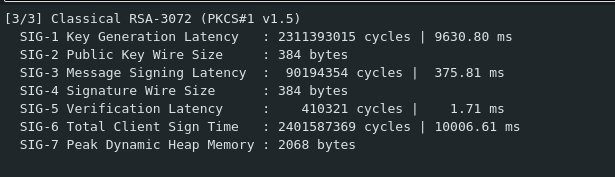
\includegraphics[width=0.85\textwidth]{screenshots/terminal_rsa.png}
\caption{ESP32 Serial Output for Classical RSA-3072 micro-benchmarks (240 MHz).}
\label{fig:term_rsa}
\end{figure}

\subsection{Automated Benchmark Results Summary Table Capture}

Figure~\ref{fig:term_summary} displays the automated console summary table printed at the conclusion of all micro-benchmarks.

\begin{figure}[htbp]
\centering
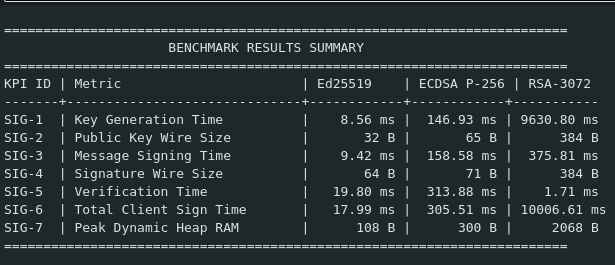
\includegraphics[width=0.85\textwidth]{screenshots/terminal_summary_table.png}
\caption{ESP32 Serial Output showing the automated Benchmark Results Summary Table.}
\label{fig:term_summary}
\end{figure}

\section{Graphical Benchmark Visualizations}

The figures below provide graphical comparisons across execution latencies, communication overheads, and dynamic memory footprints:

\subsection{Execution Latency Comparison}

Figure~\ref{fig:plot_timing} compares key generation, signing, verification, and total client sign latency on a logarithmic scale.

\begin{figure}[htbp]
\centering
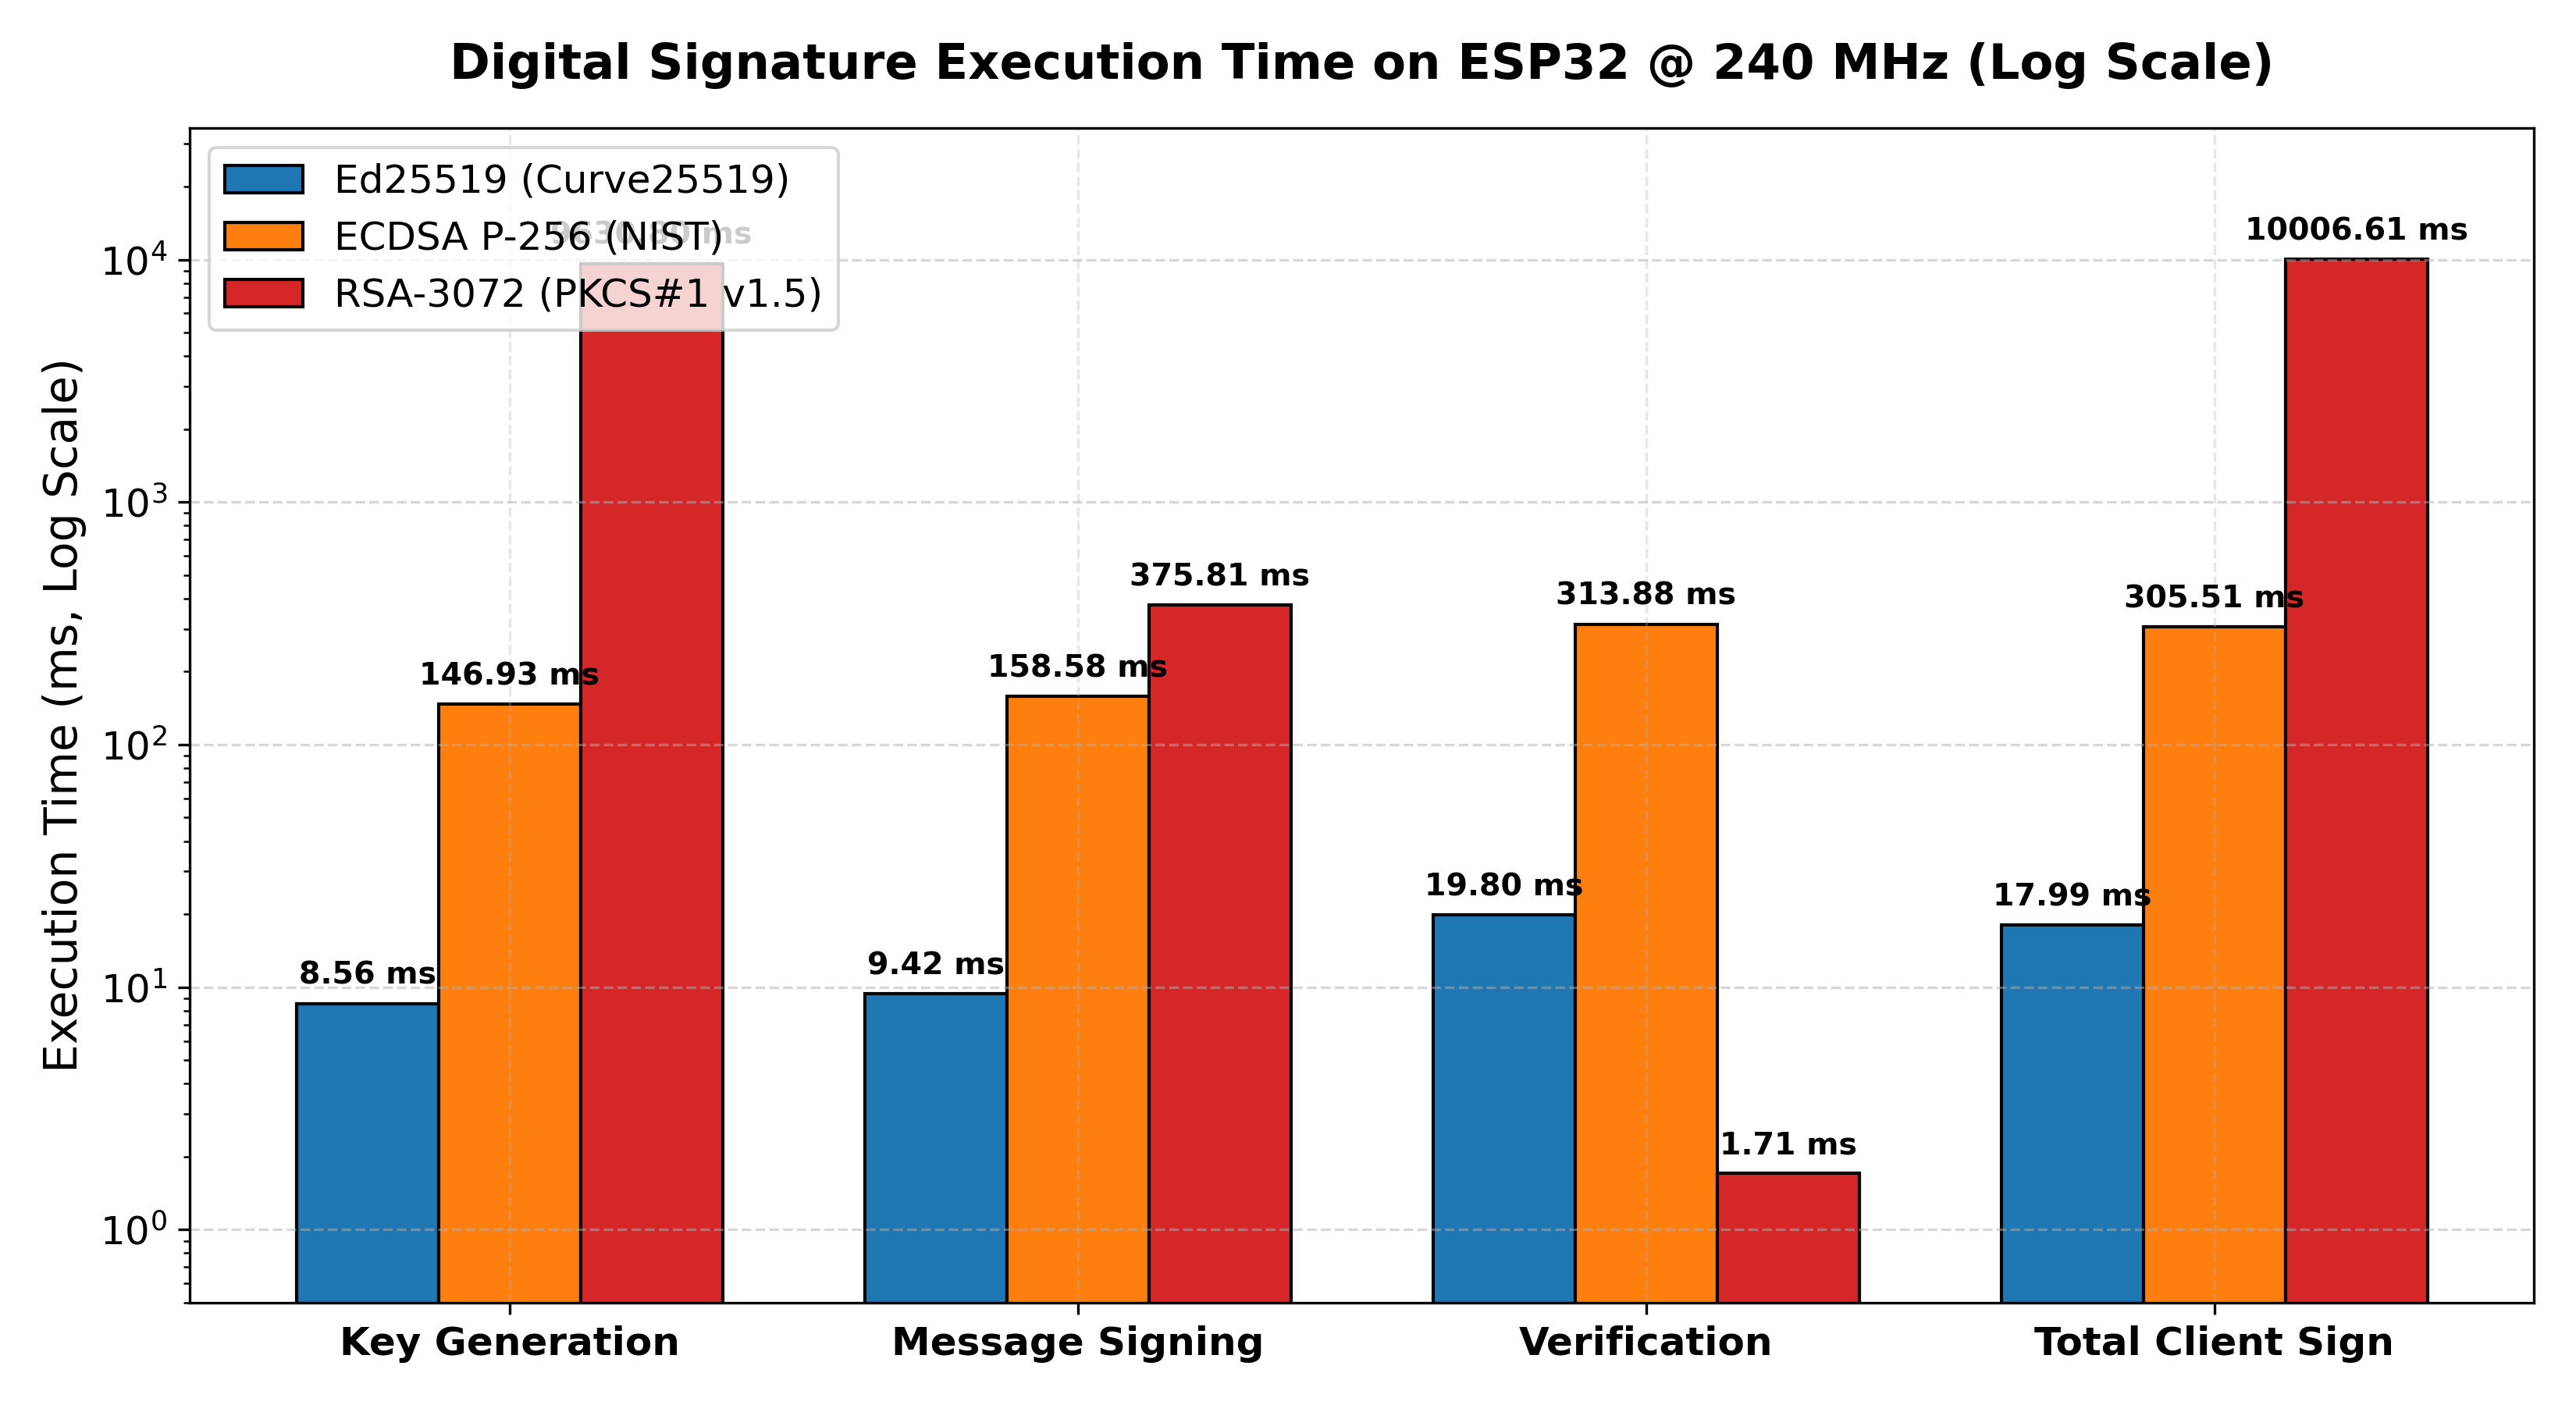
\includegraphics[width=0.82\textwidth]{graphs/fig_timing_comparison.png}
\caption{Execution latency comparison (logarithmic scale) for KeyGen, Signing, Verification, and Total Client Sign Time.}
\label{fig:plot_timing}
\end{figure}

\subsection{Communication Wire Overhead}

Figure~\ref{fig:plot_wire} breaks down the wire overhead required per mutual authentication exchange (Public Key + Signature size in bytes).

\begin{figure}[htbp]
\centering
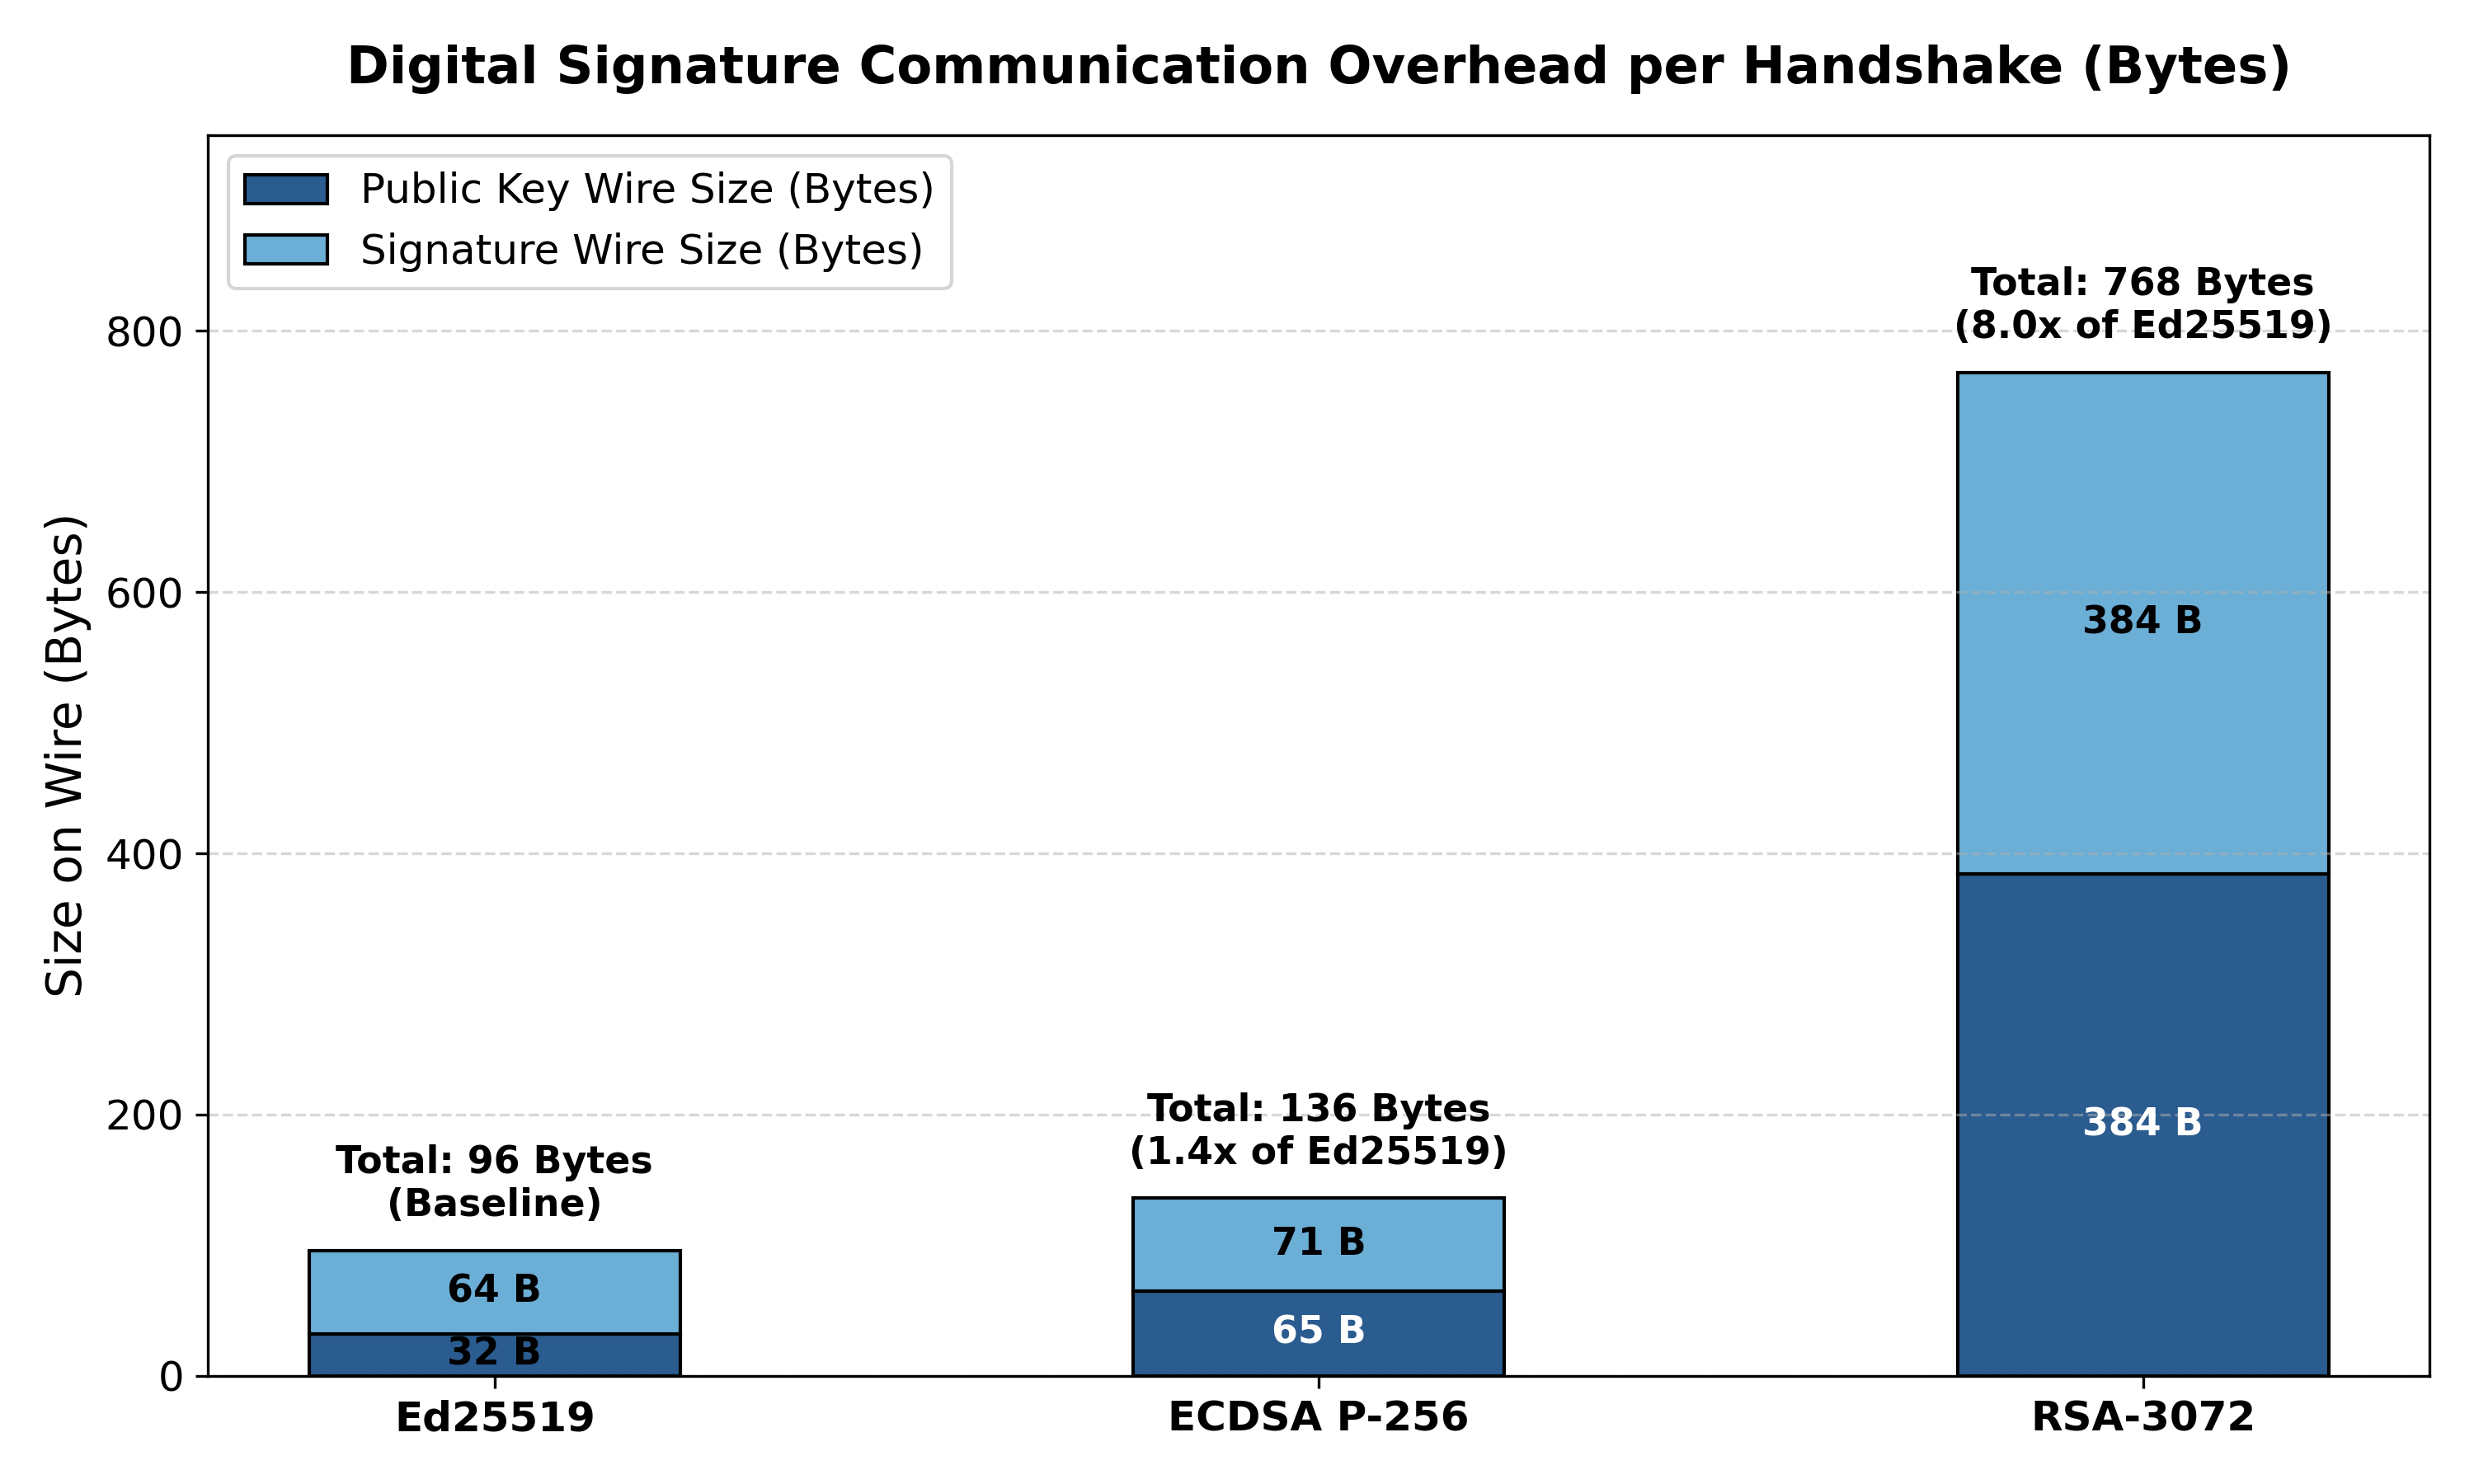
\includegraphics[width=0.78\textwidth]{graphs/fig_size_overhead.png}
\caption{Digital signature communication wire overhead per authentication handshake (Bytes).}
\label{fig:plot_wire}
\end{figure}

\subsection{Peak Dynamic Heap RAM Overhead}

Figure~\ref{fig:plot_memory} compares the peak dynamic heap memory consumed during algorithm execution on the ESP32.

\begin{figure}[htbp]
\centering
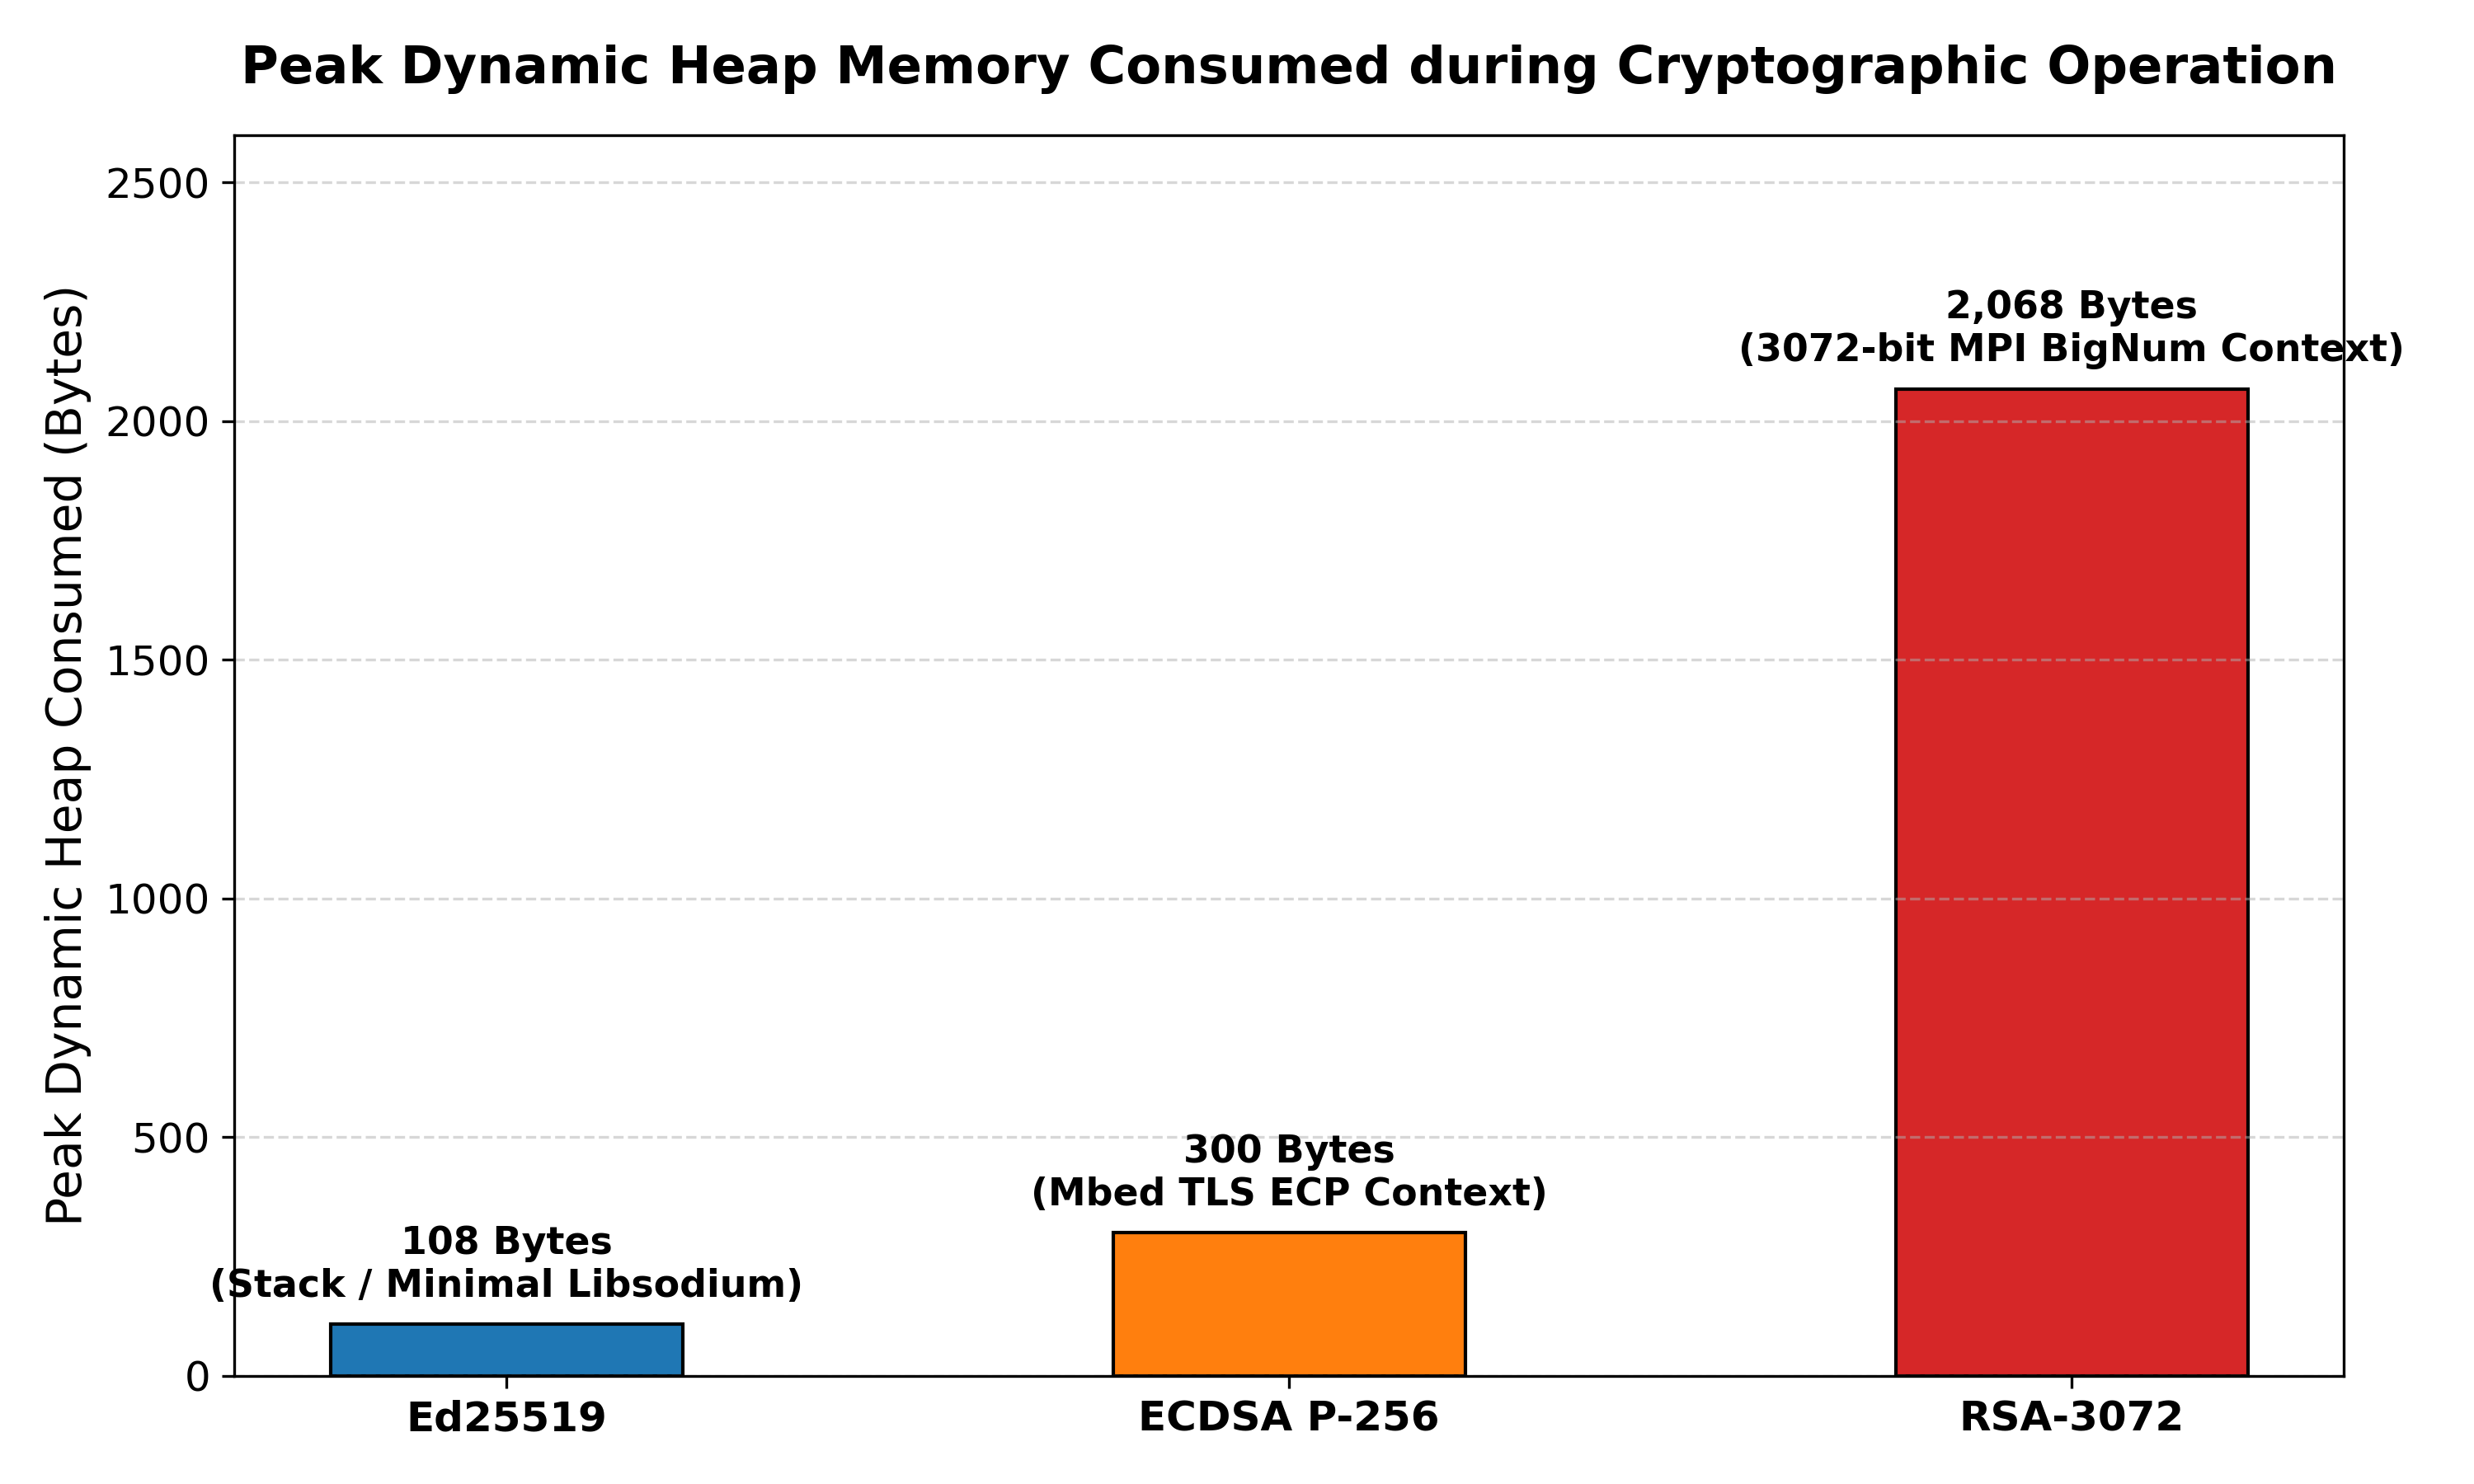
\includegraphics[width=0.78\textwidth]{graphs/fig_memory_comparison.png}
\caption{Peak dynamic heap memory allocation during digital signature execution on the ESP32.}
\label{fig:plot_memory}
\end{figure}

\section{Benchmarking Logic and Pseudocode}

The pseudocode below details the exact measurement routines implemented on the ESP32 firmware, covering cycle-accurate timers, heap profiling, and test loops for all three algorithms:

\subsection{Hardware Measurement Helpers}

\begin{lstlisting}[language=C++]
// Configuration: ESP32 runs at 240 MHz clock speed
#define FAST_RUNS      100
#define SLOW_RSA_RUNS  10
#define FAST_RSA_RUNS  100
#define MSG_SIZE       64
#define CPU_SPEED      240

// Direct read of the 32-bit hardware cycle register (ccount)
static inline uint32_t get_cycles() {
  uint32_t cycles;
  __asm__ __volatile__("rsr %0, ccount" : "=a"(cycles));
  return cycles;
}

// Convert raw CPU clock cycles into milliseconds
float cycles_to_ms(uint32_t cycles) {
  return (float)cycles / (CPU_SPEED * 1000.0f);
}
\end{lstlisting}

\subsection{Ed25519 Micro-Benchmark Routine}

\begin{lstlisting}[language=C++]
// Target KPIs: SIG-1 (KeyGen), SIG-2 (Wire: 32 B), SIG-3 (Signing), SIG-4 (Sig: 64 B),
//              SIG-5 (Verify), SIG-6 (Total Client Sign), SIG-7 (Heap: 108 B)
uint8_t public_key[crypto_sign_PUBLICKEYBYTES];   // [SIG-2] 32 bytes
uint8_t private_key[crypto_sign_SECRETKEYBYTES];
uint8_t signature[crypto_sign_BYTES];             // [SIG-4] 64 bytes
unsigned long long sig_length = 0;

uint32_t heap_before = ESP.getFreeHeap();
uint32_t peak_heap = 0;

for (int i = 0; i < FAST_RUNS; i++) {
  // [SIG-1] Key Generation Latency (8.56 ms | 2,055,308 cycles)
  uint32_t start = get_cycles();
  crypto_sign_keypair(public_key, private_key);
  time_keygen[i] = get_cycles() - start;

  // [SIG-7] Peak Dynamic Heap Profiling (108 bytes)
  uint32_t used = heap_before - ESP.getFreeHeap();
  if (used > peak_heap) peak_heap = used;

  // [SIG-3] Message Signing Latency (9.42 ms | 2,261,378 cycles)
  start = get_cycles();
  crypto_sign_detached(signature, &sig_length, test_message, MSG_SIZE, private_key);
  time_sign[i] = get_cycles() - start;

  // [SIG-5] Verification Latency (19.80 ms | 4,750,949 cycles)
  start = get_cycles();
  crypto_sign_verify_detached(signature, test_message, MSG_SIZE, public_key);
  time_verify[i] = get_cycles() - start;

  // [SIG-6] Total Client Sign Time = SIG-1 + SIG-3 (17.99 ms | 4,316,686 cycles)
}
\end{lstlisting}

\subsection{ECDSA P-256 Micro-Benchmark Routine}

\begin{lstlisting}[language=C++]
// Target KPIs: SIG-1 (KeyGen), SIG-2 (Wire: 65 B), SIG-3 (Signing), SIG-4 (Sig: 71 B),
//              SIG-5 (Verify), SIG-6 (Total Client Sign), SIG-7 (Heap: 300 B)
mbedtls_ecdsa_context main_key;
mbedtls_ecdsa_init(&main_key);
mbedtls_ecdsa_genkey(&main_key, MBEDTLS_ECP_DP_SECP256R1, mbedtls_ctr_drbg_random, &random_gen);

uint8_t signature[MBEDTLS_ECDSA_MAX_LEN];
size_t sig_length = 0;

uint32_t heap_before = ESP.getFreeHeap();
uint32_t peak_heap = 0;

for (int i = 0; i < FAST_RUNS; i++) {
  // [SIG-1] Key Generation Latency (146.93 ms | 35,262,354 cycles)
  mbedtls_ecdsa_context temp_key;
  mbedtls_ecdsa_init(&temp_key);
  uint32_t start = get_cycles();
  mbedtls_ecdsa_genkey(&temp_key, MBEDTLS_ECP_DP_SECP256R1, mbedtls_ctr_drbg_random, &random_gen);
  time_keygen[i] = get_cycles() - start;

  // [SIG-7] Peak Dynamic Heap Profiling (Captures ECP context allocation: 300 bytes)
  uint32_t used = heap_before - ESP.getFreeHeap();
  if (used > peak_heap) peak_heap = used;
  mbedtls_ecdsa_free(&temp_key);

  // [SIG-3] Message Signing Latency (158.58 ms | 38,059,479 cycles)
  // [SIG-4] Signature Wire Size (71 bytes DER sequence)
  sig_length = 0;
  start = get_cycles();
  mbedtls_ecdsa_write_signature(&main_key, MBEDTLS_MD_SHA256, message_hash, 32,
                                signature, sizeof(signature), &sig_length,
                                mbedtls_ctr_drbg_random, &random_gen);
  time_sign[i] = get_cycles() - start;

  // [SIG-5] Verification Latency (313.88 ms | 75,331,369 cycles)
  start = get_cycles();
  mbedtls_ecdsa_read_signature(&main_key, message_hash, 32, signature, sig_length);
  time_verify[i] = get_cycles() - start;

  // [SIG-6] Total Client Sign Time = SIG-1 + SIG-3 (305.51 ms | 73,321,833 cycles)
}
\end{lstlisting}

\subsection{Classical RSA-3072 Micro-Benchmark Routine}

\begin{lstlisting}[language=C++]
// Target KPIs: SIG-1 (KeyGen), SIG-2 (Wire: 384 B), SIG-3 (Signing), SIG-4 (Sig: 384 B),
//              SIG-5 (Verify), SIG-6 (Total Client Sign), SIG-7 (Heap: 2068 B)
mbedtls_pk_context main_key;
mbedtls_pk_init(&main_key);
mbedtls_pk_setup(&main_key, mbedtls_pk_info_from_type(MBEDTLS_PK_RSA));
mbedtls_rsa_gen_key(mbedtls_pk_rsa(main_key), mbedtls_ctr_drbg_random, &random_gen, 3072, 65537);

uint8_t signature[384];   // [SIG-4] 384 bytes
size_t sig_length = 0;

uint32_t heap_before = ESP.getFreeHeap();
uint32_t peak_heap = 0;

// [SIG-1] RSA Key Generation Loop (10 runs, 9,630.80 ms | 2,311,393,015 cycles)
for (int i = 0; i < SLOW_RSA_RUNS; i++) {
  mbedtls_pk_context temp_key;
  mbedtls_pk_init(&temp_key);
  mbedtls_pk_setup(&temp_key, mbedtls_pk_info_from_type(MBEDTLS_PK_RSA));

  uint32_t start = get_cycles();
  mbedtls_rsa_gen_key(mbedtls_pk_rsa(temp_key), mbedtls_ctr_drbg_random, &random_gen, 3072, 65537);
  time_keygen[i] = get_cycles() - start;

  // [SIG-7] Peak Dynamic Heap Profiling (Captures 3072-bit BigNum MPI context: 2,068 bytes)
  uint32_t used = heap_before - ESP.getFreeHeap();
  if (used > peak_heap) peak_heap = used;

  mbedtls_pk_free(&temp_key);
  vTaskDelay(1); // Yield to prevent Watchdog Timeout
}

// [SIG-3] RSA Signing Loop (100 runs, 375.81 ms | 90,194,354 cycles)
for (int i = 0; i < FAST_RSA_RUNS; i++) {
  sig_length = 0;
  uint32_t start = get_cycles();
  mbedtls_pk_sign(&main_key, MBEDTLS_MD_SHA256, message_hash, 32,
                  signature, sizeof(signature), &sig_length,
                  mbedtls_ctr_drbg_random, &random_gen);
  time_sign[i] = get_cycles() - start;
  if (i % 10 == 0) vTaskDelay(1);
}

// [SIG-5] RSA Verification Loop (100 runs, 1.71 ms | 410,321 cycles)
for (int i = 0; i < FAST_RSA_RUNS; i++) {
  uint32_t start = get_cycles();
  mbedtls_pk_verify(&main_key, MBEDTLS_MD_SHA256, message_hash, 32, signature, sig_length);
  time_verify[i] = get_cycles() - start;
}

// [SIG-6] Total Client Sign Time = SIG-1 + SIG-3 (10,006.61 ms | 2,401,587,369 cycles)
\end{lstlisting}

\end{document}
